
\chapter{Arduino Cicuit Design}
\section{Establish Connection}
\begin{figure}[H]
 \centering
    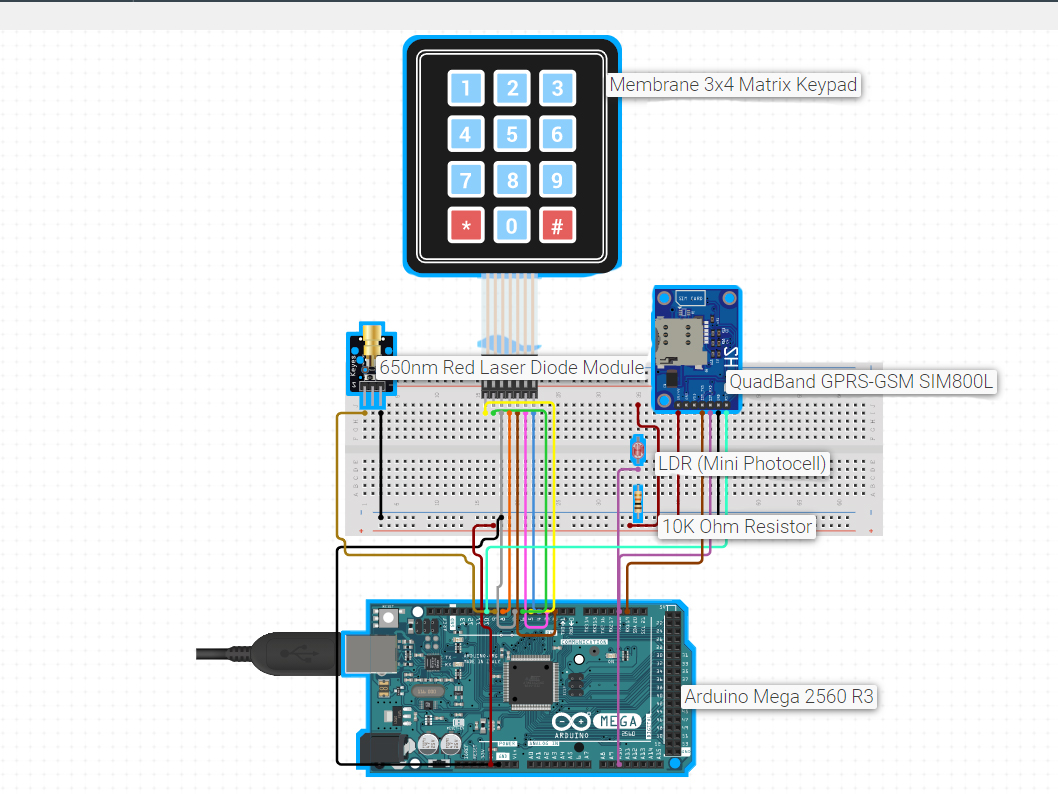
\includegraphics[height= 10cm, width=13cm]{project/images/circuit diagram}
  \caption{\textbf{Arduino Cicuit Design}}
\end{figure}
\paragraph{}1. We use SIM900 GSM Module – This means the module supports communication in 900MHz band. We are from India and most of the mobile network providers in this country operate in the 900Mhz band. If you are from another country, you have to check the mobile network band in your are
\paragraph{}2.Check the power requirements of GSM module – GSM modules are manufactured by different companies. They all have different input power supply specs. You need to double check your GSM modules power requirements.
\paragraph{}3.Our gsm module requires a 12 volts input. So we feed it using a 12V,1A DC power supply. I have seen gsm modules which require 15 volts and some other types which needs only 5 volts input. They differ with manufacturers. If you are having a 5V module, you can power it directly from Arduino’s 5V out.
\paragraph{}4.Check for TTL Output Pins in the module – You can feed the data from gsm module directly to Arduino only if the module is enabled with TTL output pins. Otherwise you have to convert the RS232 data to TTL using MAX232 IC and feed it to Arduino. Most of the gsm modules in market are equipped with TTL output pins. Just ensure you are buying the right one.
\paragraph{}
\textbf{Booting the GSM Module}
\paragraph{}1. Insert the SIM card to GSM module and lock it.

\paragraph{}2.Connect the adapter to GSM module and turn it ON!

\paragraph{}3.Now wait for some time (say 1 minute) and see the blinking rate of ‘status LED’  or ‘network LED’ (GSM module will take some time to establish connection with mobile network)

\paragraph{}4.Once the connection is established successfully, the status/network LED will blink continuously every 3 seconds.
\begin{figure}[H]
 \centering
    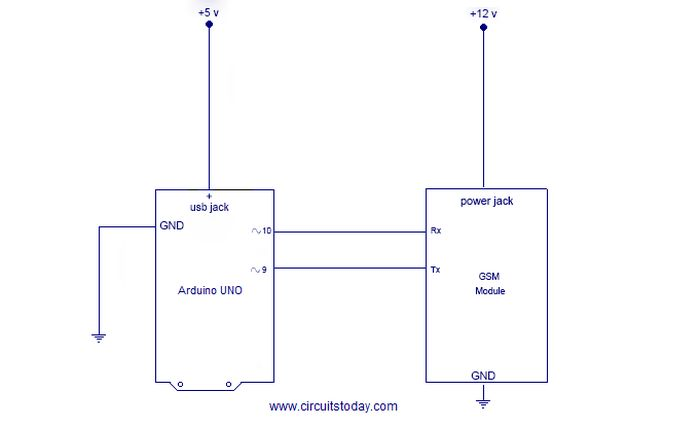
\includegraphics[height= 7cm, width=9cm]{project/images/cir}
  \caption{\textbf{Arduino and GSM Module Block Daigram}}
\end{figure}
\paragraph{}

\textbf{\\Other Connection}
\paragraph{} 1)GSM Module TXD pin in Connect to the Digital pin no 2 
\paragraph{} 2)GSM Module RXD pin in Connect to the Digital pin no 3 
\paragraph{}
\textbf{A)Buzzer Connection}
\paragraph{}1)Connnect Positive pin of Buzzer to the Digital pin no 12
\paragraph{}2)Connnect Negative pin of Buzzer to the Digital pin 3.3v
\paragraph{}
\textbf{B)Lazer Connection}
\paragraph{}1)Connnect Pin Ground to Ground
\paragraph{}2)Connnect VCC in 5v
\paragraph{}
\textbf{C)Keypad Connection}
\paragraph{}
\begin{table}[H]
\centering
\begin{tabular}{|c|c|}
\hline
4 X 4 Keypad & Arduino           \\ \hline
R1           & \textbf{$\sim$11} \\ \hline
R2           & \textbf{$\sim$10} \\ \hline
\textbf{R3}  & \textbf{$\sim$9}  \\ \hline
\textbf{R4}  & \textbf{8}        \\ \hline
\textbf{C1}  & \textbf{7}        \\ \hline
\textbf{C2}  & \textbf{$\sim$6}  \\ \hline
\textbf{C3}  & \textbf{$\sim$5}  \\ \hline
\textbf{C4}  & \textbf{4}        \\ \hline
\end{tabular}
\caption{Connection of Keypad and Arduino}
\end{table}


